\documentclass[a4paper,12pt]{article}

%%% Работа с русским языком
\usepackage{cmap}					% поиск в PDF
\usepackage{mathtext} 				% русские буквы в формулах
\usepackage[T2A]{fontenc}			% кодировка
\usepackage[utf8]{inputenc}			% кодировка исходного текста
\usepackage[english,russian]{babel}	% локализация и переносы
\usepackage{xcolor}
\usepackage{hyperref}
 % Цвета для гиперссылок
\definecolor{linkcolor}{HTML}{799B03} % цвет ссылок
\definecolor{urlcolor}{HTML}{799B03} % цвет гиперссылок

\hypersetup{pdfstartview=FitH,  linkcolor=linkcolor,urlcolor=urlcolor, colorlinks=true}

%%% Дополнительная работа с математикой
\usepackage{amsfonts,amssymb,amsthm,mathtools} % AMS
\usepackage{amsmath}
\usepackage{icomma} % "Умная" запятая: $0,2$ --- число, $0, 2$ --- перечисление

%% Номера формул
%\mathtoolsset{showonlyrefs=true} % Показывать номера только у тех формул, на которые есть \eqref{} в тексте.

%% Шрифты
\usepackage{euscript}	 % Шрифт Евклид
\usepackage{mathrsfs} % Красивый матшрифт

%% Свои команды
\DeclareMathOperator{\sgn}{\mathop{sgn}}

%% Перенос знаков в формулах (по Львовскому)
\newcommand*{\hm}[1]{#1\nobreak\discretionary{}
{\hbox{$\mathsurround=0pt #1$}}{}}
% графика
\usepackage{graphicx}
\graphicspath{{pictures/}}
\DeclareGraphicsExtensions{.pdf,.png,.jpg}
\author{Бурмашев Григорий, БПМИ-208}
\title{ТВиМС, дз -- 6}
\date{\today}
\begin{document}
\maketitle
\clearpage
\section*{Номер 3}
\subsection*{б) геометрическое распределение с параметром $p$}
\begin{center}
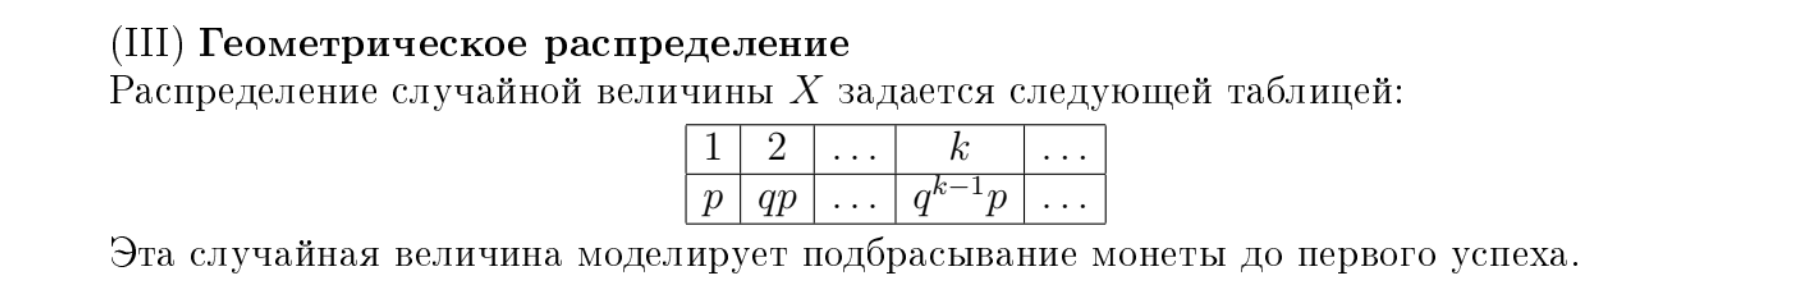
\includegraphics[scale=0.5]{1.png}
\end{center}
Найдем $\mathbb{E}X$, мы работаем с вероятностями, поэтому $q < 1, p < 1$:
\[
\mathbb{E}X = \sum_{k = 1}^{\infty} p \cdot q^{k-1} k = 
 p + 2pq + 3pq^2 + \ldots = (1-q) + 2(1-q)q + 3(1-q)q^2 + \ldots  =
\]
\[
= 
1 - q + 2q - 2q^2 + 3q^2 - 3q^3 + \ldots = 1 + q + q^2 + q^3 + \ldots = \frac{1}{1-q} = \frac{1}{p}
\]
Найдем $\mathbb{D}X$:
\[
\mathbb{D}X = \mathbb{E}X^2  - \left(\mathbb{E}X\right)^2
\]
\[
\mathbb{E}X^2 =  \sum_{k = 1}^{\infty} p \cdot q^{k-1} k^2  = p + 4pq + 9pq^2 + \ldots = (1-q) + 4(1-q)q + 9(1-q)q^2 = 
\]
\[
= 
1 - q + 4q - 4q^2 + 9q^2 - 9q^3 + \ldots = 1 + 3q + 5q^2 + \ldots = 1 + q + q^2 + q^3 + \ldots + 
\]
\[
+ 2q + 4q^2 + \ldots =  1 + q + q^2 + q^3 + \ldots + 2q(1 + q + q^2 + \ldots) + 2q^2(1 + q + q^2 + \ldots) + \ldots = 
\]
\[
=
(1 + 2q + 2q^2 + \ldots ) \cdot (1 + q + q^2 + \ldots) = (1 + 2q + 2q^2 + \ldots) \cdot \frac{1}{1-q} = \left(1 + \frac{2q}{1-q}\right) \cdot \frac{1}{1-q} =
\]
\[
=
 \frac{1}{1-q} + \frac{2q}{(1-q)^2} = \frac{2q}{p^2} + \frac{1}{p}
\]
Итого:
\[
\mathbb{D}X = \frac{2q}{p^2} + \frac{1}{p} - \frac{1}{p^2} = \frac{2 - 2p + p - 1}{p^2}= \frac{1-p}{p^2}
\]
Найдем $\mathbb{E}e^X$:
\[
\sum_{k = 1}^{\infty} p \cdot q^{k-1} e^k = pe + pqe^2 + pq^2e^3 + pq^3e^4 + \ldots = 1 = \frac{ep}{1-eq} = 
\]
\[
=
\frac{ep}{1 - e(1-p)}
\]
\begin{center}
\textbf{Ответ: } 
\[
\mathbb{EX} = \frac{1}{p}
\]
\[
\mathbb{DX} = \frac{1-p}{p^2}
\]
\[
\mathbb{E}e^X = \frac{ep}{1 - e(1-p)}
\]
\end{center}
\clearpage
\section*{Номер 9}
Боб:
\begin{center}
\begin{tabular}{|c|c|c|c|c|c|}
\hline
 $X$&$0$  &$1$  &  $2$&  $3$&$4$  \\
\hline
 $P$&  $\frac15$&   $\frac15$&  $\frac15$ &  $\frac15$ & $\frac15$  \\
\hline
\end{tabular}
\end{center}
Алиса:
\begin{center}
\begin{tabular}{|c|c|c|c|c|c|}
\hline
 $Y$&$0$  &$1$  &  $2$&  $3$&$4$  \\
\hline
 $P$&  $\frac15 \cdot \frac 12 + \frac15 \cdot \frac12 = \frac15$&   $\frac15$&  $\frac15$ &  $\frac15$ & $\frac15$  \\
\hline
\end{tabular}
\end{center}
Совместное распределение:

Алиса с вероятностью $\frac12$ отнимет от числа Боба единичку, и с такой же вероятностью прибавит. Для каждого числа Боба у Алисы будет всего 2 возможных исхода ($\pm 1$), а вероятности всех остальных равны 0.
\begin{center}
\begin{tabular}{|c|c|c|c|c|c|}
\hline
 $\frac{X}{Y}$& $0$ &  $1$& $2$ &  $3$& $4$ \\
\hline
 $0$& 0&  $\frac{1}{10}$&  0&  0& $\frac{1}{10}$ \\
\hline
$1$ &$\frac{1}{10}$ &  0&  $\frac{1}{10}$&  0& 0 \\
\hline
$2$ &  0&  $\frac{1}{10}$& 0 &  $\frac{1}{10}$&  0\\
\hline
$3$ & 0 &  0&  $\frac{1}{10}$&  0&  $\frac{1}{10}$\\
\hline
 $4$&  $\frac{1}{10}$&  0& 0 & $\frac{1}{10}$ & 0\\
\hline
\end{tabular}
\end{center}
\clearpage
\section*{Номер 10}
\subsection*{а)}
Пусть $P(X = \alpha) = p$, тогда посмотрим на $P(XY = \alpha)$, у нас возможно 2 случая:
\begin{enumerate}
\item $Y = 1$:
\[
q_1 = p \cdot \frac{1}{2}
\]
\item $Y = -1$:
\[
q_2 = p \cdot \frac{1}{2}
\]
Итого:
\[
P(XY = \alpha) = q = p \cdot \frac12 \cdot 2 = p = P(X = \alpha)
\]
\end{enumerate}
\begin{center}
\textbf{Ч.Т.Д} 
\end{center}
\section*{б)}
Хотим:
\[
P(XYZ = a\; \cap\;XYW = b\; \cap\; XW = c) = P(XYZ = a) \; \cap\; P(XYW = b)\;  \cap\; P(XW = c)
\]
Для начала заметим, что:
\[
P(XW = 1) = P(XW = -1)= \frac{1}{2}
\]
Это так, потому что и для X, и для Y у нас 2 варианта ($\pm 1$), всего 4 варианта, но подходят нам всего 2 из них (только 1, 1 и -1, -1 для единички, например), остальные варианты дают другой знак.


Также нужно заметить, что:
\[
P(XYZ = 1) = P(XYZ = -1) = P(XYW = 1) = P(XYW = -1) = \frac12
\]
Аналогично предыдущему случаю, но уже для случая из 3 позиций, всего у нас 8 вариантов, а подходят нам ровно 4 (для единички это например 1,1,1; -1, -1, 1; 1, -1, -1; -1, 1, -1, аналогично для -1)

Чтобы ответ на задачу был утвердительным, нам нужно, чтобы равенство из самого начала задачи выполнялось, т.е  $P(XYZ = a\; \cap\;XYW = b\; \cap\; XW = c) =  \frac12 \cdot \frac12 \cdot \frac12 = \frac18$

Заметим, что, чтобы получить $XW = c$, мы должны рассматривать всего 2 варианта (показали выше, например 1,1 и -1, -1 для единички и -1, 1, 1, -1 для минус единички), при таком раскладе из $XYW$ мы можем однозначно определить, какой у нас будет Y (ибо в пересечении будет $X^2$ и $W^2$ и мы сможем однозначно сказать об Y), а после этого мы сможем однозначно определить $Z$ (из пересечения всех трех, т.е $XYZ$, $XYW$,  и $XW$, т.к при таком раскладе будут $X^2$, $W^2$, $Y^2$) Итого у нас будет $(\frac12 \cdot \frac12 \cdot \frac12 \cdot \frac12) + (\frac12 \cdot \frac12 \cdot \frac12 \cdot \frac12)= \frac{1}{16} + \frac{1}{16} = \frac18$
Таким образом мы получили, что:
\[
P(XYZ = a\; \cap\;XYW = b\; \cap\; XW = c) =\frac18
\]
\[
 P(XYZ = a) \; \cap\; P(XYW = b)\;  \cap\; P(XW = c) = \frac18
\]
\begin{center}
$\longrightarrow$
\end{center}
\[
P(XYZ = a\; \cap\;XYW = b\; \cap\; XW = c) =  P(XYZ = a) \; \cap\; P(XYW = b)\;  \cap\; P(XW = c)
\]
$\longrightarrow$ величины являются независимыми в совокупности
\begin{center}
\textbf{Ответ: } величины \textbf{являются }независимыми в совокупности
\end{center}
\end{document}
